\section{容量公式}
\label{sec:dcc-capacity-formula}

可达速率的定义涉及所有码长、所有码本与所有解码器，直接求其上确界无从下手。本节从信道本身构造一个可以计算的量，并证明它控制任意长度输入块能获得的信息。下一节再证明它就是$C_{\mathrm{op}}$。

\paragraph{计数的图景}
先用一个粗略的计数说明为什么应当看互信息。设输入块的各符号按分布$q$独立选取，输出块也就按$p_q$独立分布。由第~\ref{chap:lossless-coding}章的典型集合，输出块几乎总落在约$2^{nH(Y)}$个“典型”输出块之中；给定一个码字，信道噪声使输出块落在约$2^{nH(Y\mid X)}$个块组成的小范围内。若要从输出块唯一认出码字，各码字的小范围应当基本不重叠，于是码字数至多约为
\[
 \frac{2^{nH(Y)}}{2^{nH(Y\mid X)}}=2^{n\,(H(Y)-H(Y\mid X))}=2^{nI(X;Y)} .
\]
每次使用约承载$I(X;Y)$比特。图~\ref{fig:dcc-typical-fans}画出这幅图景。它是启发，不是证明：“约”字隐去了误差，小范围之间也不必完全不交。第~\ref{sec:dcc-coding-theorem}节把这个计数做成严格的论证。

\begin{BookInlineFigure}
 \centering
 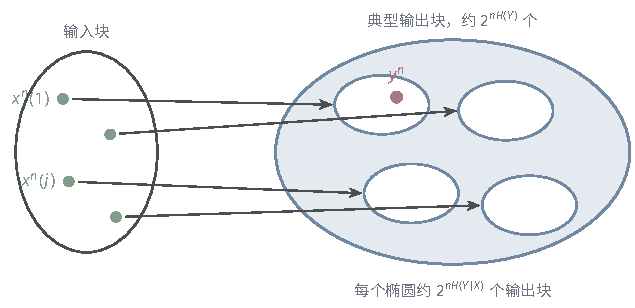
\includegraphics[width=107.5mm]{figures/07-probability/06-channel-coding/tikz/dcc-typical-fans/figure.pdf}
 \caption{容量公式背后的计数。左侧绿点是按输入分布选出的码字；右侧蓝色区域是约$2^{nH(Y)}$个典型输出块，每个码字经过信道后的可能输出集中在约$2^{nH(Y\mid X)}$个块组成的小椭圆中。红点是收到的输出块，它落在所发码字的椭圆内。互不重叠的椭圆至多约有$2^{nI(X;Y)}$个。}
 \label{fig:dcc-typical-fans}
\end{BookInlineFigure}

\paragraph{互信息作为输入分布的函数}
固定信道$\bm{W}$，输入分布为$q$时，第~\ref{chap:information-measures}章的互信息（以比特计）是
\[
 I(X;Y)=\sum_{x,y}q(x)W(y\mid x)\log_2\frac{W(y\mid x)}{p_q(y)} ,
\]
求和只取$q(x)W(y\mid x)>0$的项，此时$p_q(y)\geq q(x)W(y\mid x)>0$，每项都有定义。字母表有限，所以各个熵都有限，并且$I(X;Y)=H(Y)-H(Y\mid X)$。按输入分组，内层和正是第$x$行相对于输出分布的KL散度，于是
\begin{equation}
 I(q)=\sum_{x\in\mathcal{X}}q(x)\,D_{\mathrm{KL}}\bigl(W_x\Vert p_q\bigr) .
 \label{eq:dcc-mi-divergence}
\end{equation}
这里把互信息写成$I(q)$，强调信道固定后它只是$q$的函数。式~\eqref{eq:dcc-mi-divergence}的读法是：每个输入$x$的输出分布偏离总体输出分布越远，用$x$传递的信息越多；互信息是这些偏离按使用频率的平均。

\begin{definition}[信息容量]
\label{def:dcc-information-capacity}
离散信道$\bm{W}$的信息容量是
\begin{equation}
 C=\max_{q\in\Delta_{\mathcal{X}}}I(q) .
 \label{eq:dcc-capacity}
\end{equation}
达到最大值的$q$称为最优输入分布。
\end{definition}

定义中写的是最大值而不是上确界，需要说明它能取到；同时，最优输入分布怎样刻画，也决定了后面的计算方法。

\begin{theorem}[容量的存在与凹性]
\label{thm:dcc-capacity-exists}
$I(q)$是单纯形$\Delta_{\mathcal{X}}$上的连续凹函数。因此式~\eqref{eq:dcc-capacity}的最大值存在，并且
\begin{equation}
 0\leq C\leq\min\bigl\{\log_2\lvert\mathcal{X}\rvert,\ \log_2\lvert\mathcal{Y}\rvert\bigr\} ;
 \label{eq:dcc-capacity-range}
\end{equation}
最优输入分布组成凸集，所有最优输入分布给出同一个输出分布。
\end{theorem}

\begin{proof}
把互信息写成熵差：
\[
 I(q)=H(p_q)-\sum_{x}q(x)H(W_x) ,
\]
其中$H(p_q)=\sum_y\varphi(p_q(y))$，$\varphi(t)=-t\log_2t$（$\varphi(0)=0$）。$\varphi$在$[0,1]$上连续，$p_q$是$q$的线性函数，所以$H(p_q)$关于$q$连续；第二项是$q$的线性函数。于是$I$连续。

凹性。第~\ref{chap:information-measures}章证明了熵是概率分布的凹函数，而且因为$\varphi$严格凹，这种凹性是严格的：$p\neq p'$时，对$0<\theta<1$有$H(\theta p+(1-\theta)p')>\theta H(p)+(1-\theta)H(p')$。$q\mapsto p_q$是线性的，凹函数与线性映射的复合仍是凹函数；减去一个线性函数不改变凹性。所以$I$凹。

$\Delta_{\mathcal{X}}$是有界闭集，连续函数在其上取到最大值。凹函数在凸集上的最大值点组成凸集：若$q_1,q_2$都达到$C$，则对$\theta\in[0,1]$，
\[
 I\bigl(\theta q_1+(1-\theta)q_2\bigr)\geq\theta C+(1-\theta)C=C .
\]
若两者的输出分布不同，由$H$的严格凹性，中点处的不等式是严格的，$I$会超过$C$，这不可能。所以最优输出分布唯一。

上界：$I(X;Y)\leq H(X)\leq\log_2\lvert\mathcal{X}\rvert$，同理$I(X;Y)\leq H(Y)\leq\log_2\lvert\mathcal{Y}\rvert$；下界由互信息非负得到。
\end{proof}

凹性带来的好处是局部最优就是全局最优，最优输入可以用一阶条件刻画。凹性本身不保证最优输入唯一：例如两个输入的转移行完全相同时，它们之间的分配可以任意调换。

\paragraph{例：Z信道}
Z信道中记$q=\mathbb{P}(X=1)$。输出为$1$当且仅当输入为$1$且没有出错，所以$p_q(1)=q/2$。给定$X=0$时输出确定，熵为$0$；给定$X=1$时输出是公平硬币，熵为$1$比特。于是
\[
 I(q)=h_2\Bigl(\frac q2\Bigr)-q ,
\]
其中$h_2(t)=-t\log_2t-(1-t)\log_2(1-t)$是二元熵函数。对$q$求导，$h_2'(t)=\log_2\frac{1-t}{t}$，得到
\[
 I'(q)=\frac12\log_2\frac{2-q}{q}-1 .
\]
令它为零，得$(2-q)/q=4$，即$q=\tfrac25$。代回，$h_2(\tfrac15)=\log_25-\tfrac85$，所以
\[
 C=\log_25-\frac85-\frac25=\log_2\frac54\approx0.3219 .
\]
最优输入并不均匀：输入$1$会以一半的概率被误读成$0$，少用一些更划算。均匀输入时$I(\tfrac12)=h_2(\tfrac14)-\tfrac12\approx0.3113$，比容量少约$0.011$比特。图~\ref{fig:dcc-mi-curves}把它与两个对称信道的$I(q)$画在一起。

\begin{BookInlineFigure}
 \centering
 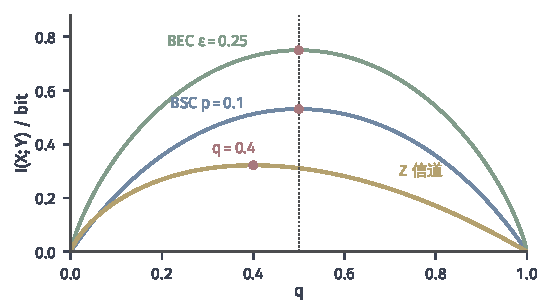
\includegraphics[width=92mm]{figures/07-probability/06-channel-coding/matplotlib/dcc-mi-curves/figure.pdf}
 \caption{三个二元输入信道的互信息随输入概率$q=\mathbb{P}(X=1)$的变化：蓝线为翻转概率$0.1$的二元对称信道，绿线为擦除概率$0.25$的二元擦除信道，黄线为Z信道。三条曲线都是凹的，红点为最大值即容量；两个对称信道在$q=\tfrac12$处取最大值，Z信道在$q=0.4$处取最大值$\log_2(5/4)$。}
 \label{fig:dcc-mi-curves}
\end{BookInlineFigure}

\paragraph{最优性条件}
对二元输入，一元求导就能找到最大值；输入多于两个时，需要一个对单纯形上的点都适用的判别法。式~\eqref{eq:dcc-mi-divergence}提示：最优时，凡是被使用的输入，其“信息贡献”$D_{\mathrm{KL}}(W_x\Vert p_q)$应当相等，否则把概率从贡献小的输入挪到贡献大的输入就能增加互信息。下面的定理把这一想法写准确，并顺带给出一个任何时候都能算的上界。

\begin{theorem}[容量的上界与最优性条件]
\label{thm:dcc-kkt}
\begin{enumerate}
 \item 对$\mathcal{Y}$上的任意概率分布$r$，
 \begin{equation}
  C\leq\max_{x\in\mathcal{X}}D_{\mathrm{KL}}\bigl(W_x\Vert r\bigr) .
  \label{eq:dcc-upper-bound}
 \end{equation}
 \item $q^{*}\in\Delta_{\mathcal{X}}$是最优输入分布，当且仅当存在常数$c$，使得记$p^{*}=p_{q^{*}}$时
 \begin{equation}
  D_{\mathrm{KL}}\bigl(W_x\Vert p^{*}\bigr)=c\ \ \text{若}\ q^{*}(x)>0,\qquad D_{\mathrm{KL}}\bigl(W_x\Vert p^{*}\bigr)\leq c\ \ \text{若}\ q^{*}(x)=0 .
  \label{eq:dcc-kkt}
 \end{equation}
 此时$c=C$。
\end{enumerate}
\end{theorem}

\begin{proof}
先证一个恒等式。对任意$q$与任意$r$，把$\log_2(W/r)$拆成$\log_2(W/p_q)+\log_2(p_q/r)$，得到
\[
 \sum_{x}q(x)D_{\mathrm{KL}}(W_x\Vert r)=\sum_xq(x)D_{\mathrm{KL}}(W_x\Vert p_q)+\sum_{y}p_q(y)\log_2\frac{p_q(y)}{r(y)} ,
\]
其中用到$\sum_xq(x)W(y\mid x)=p_q(y)$。由式~\eqref{eq:dcc-mi-divergence}，右边是$I(q)+D_{\mathrm{KL}}(p_q\Vert r)$。若某项为无穷，等式两边同为无穷。于是
\[
 I(q)=\sum_xq(x)D_{\mathrm{KL}}(W_x\Vert r)-D_{\mathrm{KL}}(p_q\Vert r)\leq\max_xD_{\mathrm{KL}}(W_x\Vert r) .
\]
对$q$取最大值就得到式~\eqref{eq:dcc-upper-bound}。

充分性。设式~\eqref{eq:dcc-kkt}成立。由式~\eqref{eq:dcc-mi-divergence}，$I(q^{*})$是$D_{\mathrm{KL}}(W_x\Vert p^{*})$在$q^{*}$支撑上的平均，等于$c$。取$r=p^{*}$，式~\eqref{eq:dcc-upper-bound}给出$C\leq c$。所以$I(q^{*})=c\geq C$，$q^{*}$最优且$c=C$。

必要性。设$q^{*}$最优，任取$x'\in\mathcal{X}$，令$q_t=(1-t)q^{*}+t\,\delta_{x'}$，$t\in[0,1]$，其中$\delta_{x'}$是集中在$x'$的分布。先设$W_{x'}$的支撑包含在$p^{*}$的支撑中。对$I(q_t)=H(p_{q_t})-\sum_xq_t(x)H(W_x)$在$t=0$处求右导数，$p_{q_t}=p^{*}+t(W_{x'}-p^{*})$，熵项的导数是
\[
 \begin{aligned}
 &-\sum_{y}\bigl(W(y\mid x')-p^{*}(y)\bigr)\Bigl(\log_2p^{*}(y)+\frac{1}{\ln2}\Bigr)\\
 &\qquad=-\sum_yW(y\mid x')\log_2p^{*}(y)-H(p^{*}) ,
 \end{aligned}
\]
这里只对$p^{*}(y)>0$的$y$求和，$\sum_y(W(y\mid x')-p^{*}(y))=0$消去了常数项。线性项的导数是$-H(W_{x'})+\sum_xq^{*}(x)H(W_x)$。两部分相加，得到
\[
 \frac{\mathrm{d}}{\mathrm{d}t}I(q_t)\Big|_{t=0^{+}}=D_{\mathrm{KL}}(W_{x'}\Vert p^{*})-I(q^{*}) .
\]
$q^{*}$是最大值点，右导数不能为正，所以$D_{\mathrm{KL}}(W_{x'}\Vert p^{*})\leq I(q^{*})=C$。若$W_{x'}$在某个$p^{*}(y)=0$的$y$上有正质量，则$p_{q_t}(y)=tW(y\mid x')$，熵中这一项$-tW\log_2(tW)$的右导数为$+\infty$，其余项导数有限，$I(q_t)$在$t=0$附近严格增加，与最优性矛盾；所以这种情形不会出现。于是对一切$x'$有$D_{\mathrm{KL}}(W_{x'}\Vert p^{*})\leq C$；而这些散度按$q^{*}$的平均等于$C$，所以在支撑上必须取等号。
\end{proof}

式~\eqref{eq:dcc-kkt}是卷五中约束优化一阶条件在单纯形上的具体形式：等式约束$\sum_xq(x)=1$的乘子是$c$，非负约束在$q^{*}(x)=0$处起作用，允许不等号，可参考\BookChapterRef{chap:constrained-optimality}{卷五第17章“约束问题的最优性”}。上界~\eqref{eq:dcc-upper-bound}对任意$r$成立，不需要知道最优输入；第~\ref{sec:dcc-numerical}节用它作为数值计算的停止依据。

用Z信道检验条件~\eqref{eq:dcc-kkt}。$q^{*}=(\tfrac35,\tfrac25)$时$p^{*}=(\tfrac45,\tfrac15)$，两行的散度为
\[
 \begin{aligned}
 D_{\mathrm{KL}}(W_0\Vert p^{*})&=\log_2\frac{1}{4/5}=\log_2\frac54 ,\\
 D_{\mathrm{KL}}(W_1\Vert p^{*})&=\frac12\log_2\frac{1/2}{4/5}+\frac12\log_2\frac{1/2}{1/5}=\frac12\log_2\frac{25}{16}=\log_2\frac54 .
 \end{aligned}
\]
两者相等，都等于容量。

\paragraph{块的互信息不超过单次容量的$n$倍}
容量是单次使用的量，传输却用整块输入。块输入的各符号可以按任意方式相关，例如重复码让三个符号完全相同。这种相关能否让$n$次使用获得多于$nC$的信息？下面的引理说不能，并且独立使用最优输入恰好达到$nC$。

\begin{lemma}[块互信息的单次上界]
\label{lem:dcc-block-bound}
设$X^n=(X_1,\dots,X_n)$在$\mathcal{X}^n$上有任意分布，给定$X^n=x^n$时$Y^n$的条件分布由式~\eqref{eq:dcc-memoryless}给出。则
\begin{equation}
 I(X^n;Y^n)\leq\sum_{i=1}^{n}I(X_i;Y_i)\leq nC .
 \label{eq:dcc-block-bound}
\end{equation}
若$X_1,\dots,X_n$独立且都服从最优输入分布，则两处都取等号。
\end{lemma}

\begin{proof}
先算条件熵。对式~\eqref{eq:dcc-memoryless}中$j\neq i$的坐标求和，每个因子$\sum_{y_j}W(y_j\mid x_j)=1$，得到$\mathbb{P}(Y_i=y\mid X^n=x^n)=W(y\mid x_i)$：$(X_i,Y_i)$的联合分布是$X_i$的边缘分布乘以$\bm{W}$。取对数，乘积变成和：
\[
 \begin{aligned}
 H(Y^n\mid X^n)&=\mathbb{E}\bigl[-\log_2W^n(Y^n\mid X^n)\bigr]\\
 &=\sum_{i=1}^{n}\mathbb{E}\bigl[-\log_2W(Y_i\mid X_i)\bigr]=\sum_{i=1}^{n}H(Y_i\mid X_i) .
 \end{aligned}
\]
再看输出熵。由熵的链式法则与“条件化不增加熵”，
\[
 H(Y^n)=\sum_{i=1}^{n}H(Y_i\mid Y_1,\dots,Y_{i-1})\leq\sum_{i=1}^{n}H(Y_i) .
\]
两式相减，
\[
 \begin{aligned}
 I(X^n;Y^n)&=H(Y^n)-H(Y^n\mid X^n)\\
 &\leq\sum_{i=1}^{n}\bigl(H(Y_i)-H(Y_i\mid X_i)\bigr)=\sum_{i=1}^{n}I(X_i;Y_i) .
 \end{aligned}
\]
每个$I(X_i;Y_i)$是$X_i$的边缘分布对应的互信息，不超过$C$。

若$X_i$独立同服从最优分布$q^{*}$，则联合概率$\prod_iq^{*}(x_i)W(y_i\mid x_i)$分解为$n$个相同因子的乘积，$(X_i,Y_i)$相互独立，$Y_1,\dots,Y_n$也相互独立，于是$H(Y^n)=\sum_iH(Y_i)$，且每个$I(X_i;Y_i)=C$。
\end{proof}

图~\ref{fig:dcc-memoryless-graph}画出证明所用的依赖结构。条件熵能够精确相加，是因为每个输出只通过自己的输入受影响；输出熵只能放大成和，是因为各输出可能经由输入彼此相关。输入之间的相关只会让$H(Y^n)$变小，不会让信息变多：重复码的三个输出高度相关，所以三次使用得到的信息远少于$3C$。

\begin{BookInlineFigure}
 \centering
 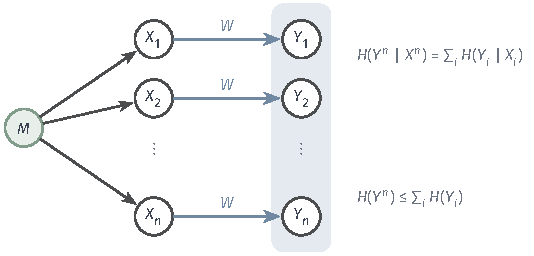
\includegraphics[width=90.5mm]{figures/07-probability/06-channel-coding/tikz/dcc-memoryless-graph/figure.pdf}
 \caption{无反馈块传输的依赖结构。消息$M$决定整个输入块，各输入可以经由$M$相关；每个输出$Y_i$只由$X_i$经过同一个$W$产生。条件熵因此精确相加，而浅蓝色框内的输出可能彼此相关，输出熵只满足次可加不等式。}
 \label{fig:dcc-memoryless-graph}
\end{BookInlineFigure}

引理只说块输入能获得的信息至多为$nC$，还没有说明这些信息能被一个码本和一个解码器实际兑现成低错误的消息传输，也没有说明信息上界为什么限制码率。这两个方向分别是下一节的可达性与逆定理。
